%=========================================================================
% (c) 2014, 2015 Josef Lusticky

\chapter{40 Gigabit Ethernet}
Previous Ethernet versions could use standard Cat 6 copper cable and RJ-45 connectors , %~\cite{10gbase-t}
whereas 40 Gigabit runs on Quad Small Form Factor Pluggable (QSPF) - a high-density fiber connector with 12 strands of fiber.

http://searchdatacenter.techtarget.com/feature/40-GbE-technology-Hurry-up-and-wait
Unlike standard two-strand fiber connections, it isn’t “field terminated,” meaning that an electrician can’t hook up a QSFP connector on site. Data center managers need to determine their cabling lengths in advance and preorder custom cables that are manufactured with the connectors already attached.


The channel layout is shown in figure~\ref{fig:40gbit-ethernet-layout}.

\begin{figure}
	\centering
	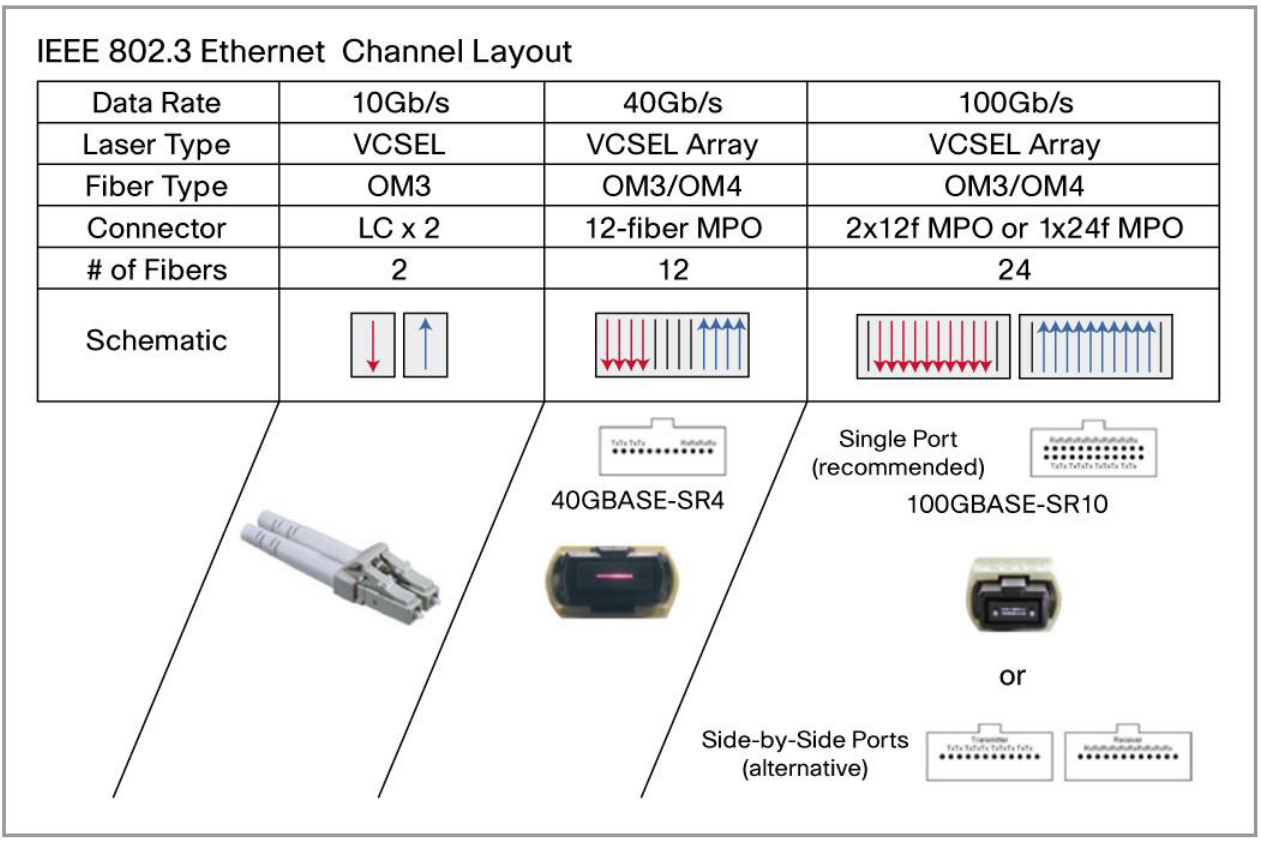
\includegraphics[width=13cm,keepaspectratio]{fig/ethernet-layout.pdf}
	\caption{IEEE 802.3 Ethernet Channel Layout (source: Cisco Systems Inc.)}
	\label{fig:40gbit-ethernet-layout}
	\bigskip
\end{figure}
